%% Estructura principal para un reporte de Trabajos intersemanales CIRCAE %%
\documentclass[conference]{IEEEtran} %tamaño del papel y el tipo de transcripción que será IEEE
\usepackage[utf8]{inputenc} %el tipo de codificación que incluye símbolos como la tilde
\usepackage[spanish]{babel} % hacemos que nuestro documentación vaya en español
\usepackage{cite} % citas bibliográficas
\usepackage{graphicx} %gráficos, usaremos solo .jpg o .png con estándares que ya veremos
\usepackage{subfigure} %usar subfiguras
\usepackage{url} %agregar direcciones url
\usepackage{amsmath} %expresiones matemáticas
\newtheorem{teor}{Teorema}[section] %definimos la enumeración de Teoremas usando la etiqueta \begin{teor} ... \end{teor} para los ejemplos, podemos darle etiquetas para referenciarlas a lo largo del texto
\newtheorem{ejem}{Ejemplo}[section] %definimos la enumeración de Ejemplos usando la etiqueta \begin{ejem} ... \end{ejem} para los ejemplos, podemos darle etiquetas para referenciarlas a lo largo del texto
\newtheorem{exper}{Experimento}[section] %definimos la enumeración de Ejemplos usando la etiqueta \begin{exper} ... \end{exper} para los Experimentos, podemos darle etiquetas para referenciarlas a lo largo del texto
\usepackage{setspace} %LA usamos para asignar el interlineado
%%%%%%% settings para incluir codigo fuente en cualquier lenguaje
\usepackage{listings} %comenzamos la configuración de nuestras lineas de codigo que se incluirá de ser necesario en el documento
\usepackage[usenames]{color} %seteamos el uso de nombre y color
\definecolor{gray97}{gray}{.97}%definimos nombre y color
\usepackage{textcomp}
\lstset{
		frame=Ltb,
		framerule=1pt,
		framextopmargin=5pt, %margen de arriba
		framexbottommargin=5pt, %margen de abajo
		framexleftmargin= -2pt, %separacion del margen izquierdo
		framesep=2pt,
		rulesep=0.2pt,
		backgroundcolor=\color{gray97},
		rulesepcolor=,
        tabsize=4,
        rulecolor=\color[RGB]{106, 182, 217}, %AZUL
        upquote=true,
        aboveskip={1.5\baselineskip}, %despues de la linea de texto
        columns=fixed,
        showstringspaces=false,
        extendedchars=true,
        breaklines=true,
        prebreak = \raisebox{0ex}[0ex][0ex]{\ensuremath{\hookleftarrow}},
        showtabs=false,
        showspaces=false,
        showstringspaces=false,
        basicstyle=\scriptsize\ttfamily\color[RGB]{39, 100, 46}, %Numeros de lineas, simbolos, puntos y coma y demas
        identifierstyle=\ttfamily\color[RGB]{56, 140, 189}, %variables
        commentstyle=\color[RGB]{62, 179, 101}, %comentarios
        stringstyle=\color[RGB]{247, 165, 42}, %impresiones
        keywordstyle=\bfseries\color[RGB]{237, 118, 150}, %funciones
        %
		numbers=left,
		numbersep=-7pt, %separacion del numero
		numberstyle=\tiny,
		numberfirstline = false,
		breaklines=true,
		}
\usepackage{graphicx}
\usepackage[colorinlistoftodos]{todonotes}
\usepackage{array}
\usepackage{fixltx2e}
%%%%%%%
\providecommand{\keywords}[1]{\textbf{\textit{Términos Clave---}} #1}

\begin{document}
\spacing{0.9} %definimos un interlineado de 0.9 para todo el documento

\title{Nombre del Proyecto en Puestión}

\author{
	\IEEEauthorblockN{\textsc{Edison Abado Anccovccccccccccccc}}
	\IEEEauthorblockA{\textit{Universidad Nacional de San}\\ \textit{Antonio abad del Cusco}\\
		Escuela profesional de \\ Ingeniería Electrónica}
	\and
	\IEEEauthorblockN{\textsc{Edison Abado Ancco}}
	\IEEEauthorblockA{\textit{Universidad Nacional de San}\\ \textit{Antonio abad del Cusco}\\
		Escuela profesional de \\ Ingeniería Electrónica}
	\and
	\IEEEauthorblockN{\textsc{Edison Abado Anccocvcvcvcvcv}}
	\IEEEauthorblockA{\textit{Universidad Nacional de San}\\ \textit{Antonio abad del Cusco}\\
		Escuela profesional de \\ Ingeniería Electrónica}
	\and
	\IEEEauthorblockN{\textsc{Edison Abado Ancco}}
	\IEEEauthorblockA{\textit{Universidad Nacional de San}\\ \textit{Antonio abad del Cusco}\\
		Escuela profesional de \\ Ingeniería Electrónica}
	\and
	\IEEEauthorblockN{\textsc{Edison Abado Ancco}}
	\IEEEauthorblockA{\textit{Universidad Nacional de San}\\ \textit{Antonio abad del Cusco}\\
		Escuela profesional de \\ Ingeniería Electrónica}
	}




\markboth{CIRCAE INFORME \today -G1-P3-005}{} % Codigo del informe que corresponde a: - numero de grupo con la G antepuesta - numero de proyecto con la P antepuesta | número de informe
\maketitle


\begin{abstract}
MicroMouse es un dispositivo en el que se aplica principios de ciencias de la computación, principios ópticos, mecánicos, electrónicos y la integración de tecnologías de software y hardware  . Lo que se pretende cubrir es la solución de un laberinto usando algoritmos de reconocimiento, almacenamiento, solución y retroalimentación con condiciones iniciales constantes en el tiempo.\\

\keywords{\textbf{Introducimos nuestros términos clave en orden alfabetico, separado por comas. Para una lista de sugerencias de palabras o términos clave visitar \underline{http://www.ieee.org/organizations/pubs/ani\_ prod/keywrd98.txt}}}
\end{abstract}

%%%%%%%%%%%%%%%%%%%%%%%%%%%%%%%%%%%%%%%%%%%%%%%
%%%%%
%%%%%   PROBLEMA     %%%%%%%%%%%%%%%%%%%%%%%%%%
%%%%%
%%%%%%%%%%%%%%%%%%%%%%%%%%%%%%%%%%%%%%%%%%%%%%%




	\section{FET de Nanotubos de Carbono}
	
	Las necesidades de eficiencia nos llevan a buscar nuevas maneras de realizar tareas con el fin de aumentar la eficiencia, partiendo de ello se tiene a un dispositivo electrónico cuya composición se gestó en 1991 por Sumio Ijima (un nanotubo multicapoa) y en 1993 con Donal Bethude que produjo nanotubos de Carbono de una sola capa.
	
	Desde entonces, se fueron desarrollando nanotubos de carbono para dierentes aplicaciones, entre ellas, la que más nos interesa, los nanotubos de carbono para aplicaciones de semiconductores, para ser más específicos, el CNFET o CNTFET (Carbon Nanotube FET) cudo diámetro de circunferencia va desde $<1nm$ hasta $50nm$ \cite{DesignandSimulationofCarbon2021} para aplicaciones de nuestro interes.
	
	
	
	\begin{figure}[h!]
		\centering
		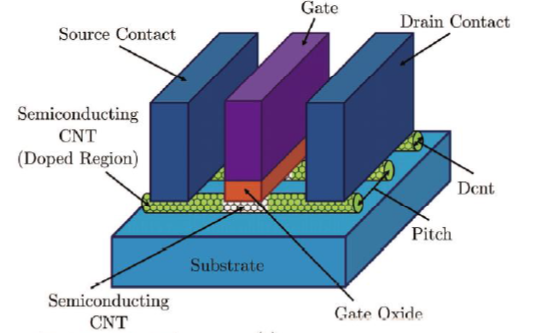
\includegraphics[width=6cm]{IMAGENES/img11}
		\caption{Diseño de un CNFET como un MOSFET \cite{DesignofanovelternarySRAM2017}}
		\label{img11}
	\end{figure}
	



	\subsection{Clasificación de nanotubos de carbono}
	
	La principal clasificación se da por el tipo de distribución de las celdas hexagonales.
	
	\begin{enumerate}
		\item Nanotubo de una sola capa (SWNT).\\
		\item Nanotubo Multicapa (MWNT). \\
		\item Nanotubo Mixto.
		
		\begin{figure}[h!]
			\centering
			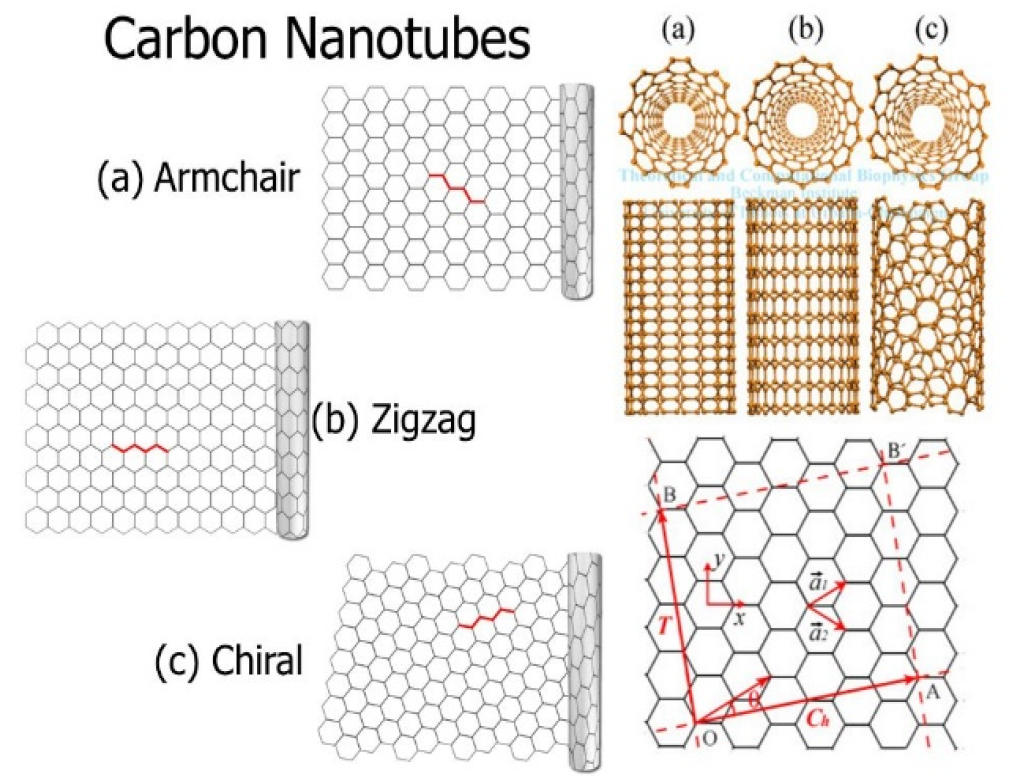
\includegraphics[width=6cm]{IMAGENES/img12}
			\caption{Los principios de construcción del CNT de planchas de grafeno \cite{PerformanceAnalysisofClassical2018} .}
			\label{img12}
		\end{figure}
		
	\end{enumerate}





	La estructura interna de CNFET es muy parecida al del MOSFET, requiere de tres pines, y también la compuerta (Gate) controla el flujo de corriente a través del canal. el switching de la compuerta habilita  la corriente del canal \cite{PerformanceAnalysisofClassical2018}. La construcción se muestra en la figura \ref{img13}
	
	\begin{figure}[h!]
		\centering
		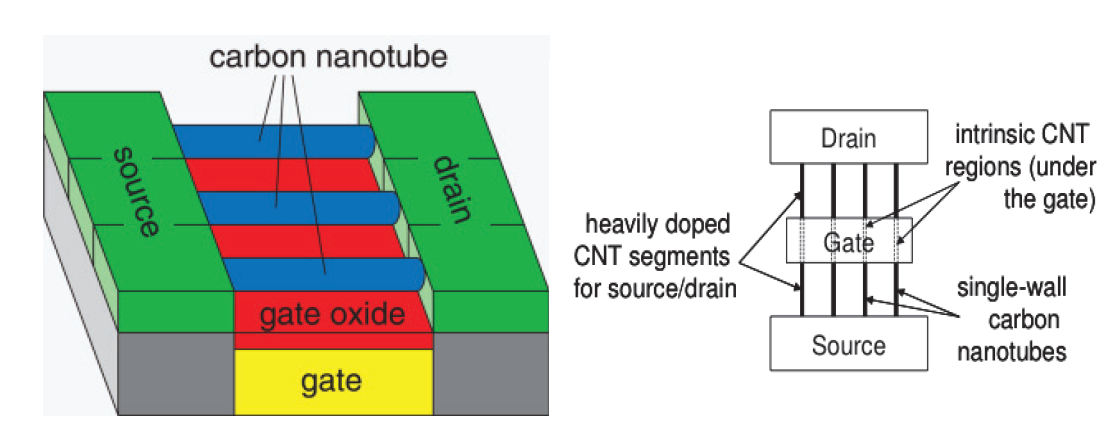
\includegraphics[width=12cm]{IMAGENES/img13}
		\caption{Estructura del CNFET \cite{Performanceinvestigationofemerging2016}.}
		\label{img13}
	\end{figure}



	\begin{figure}[h!]
		\centering
		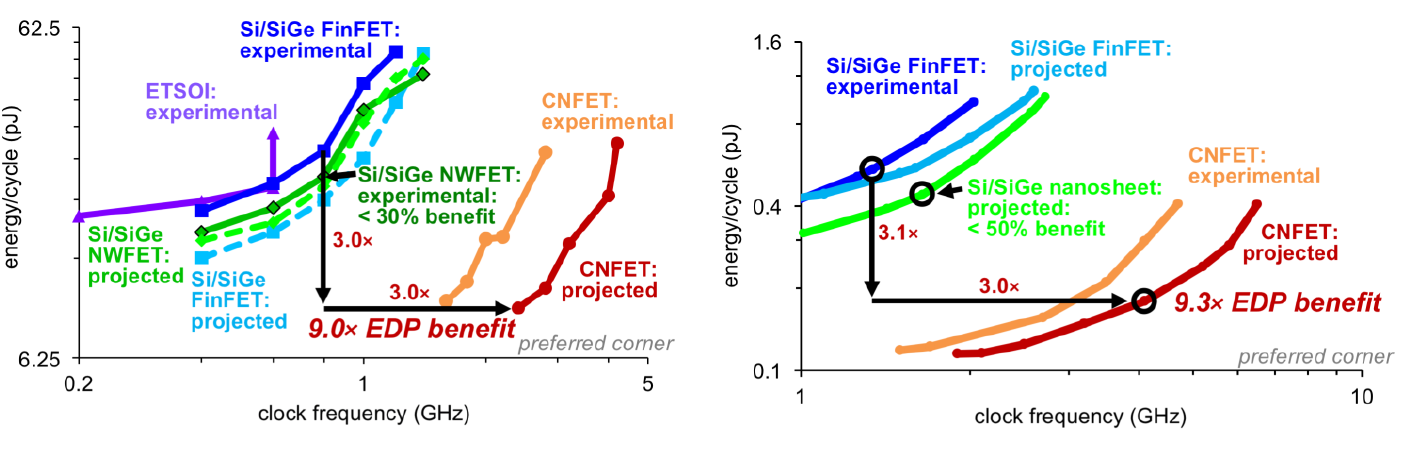
\includegraphics[width=15cm]{IMAGENES/img14}
		\caption{Comparación de otros dispositivos con CNFET de 7nm y 5nm \cite{UnderstandingEnergyEfficiency2018} .}
		\label{img14}
	\end{figure}



	\begin{table}
		\centering
		\begin{tabular}{|p{0.4\textwidth}|p{0.4\textwidth}|}
			\hline
			\begin{enumerate}
				\item[]\textbf{Nanotransistores}
				\item FET basados en nanotubos de carbono pueden operar más rápido y con un
				voltaje de suministro menor que sus equivalentes basados en silicio.
				\item Con una tensión de alimentación de 0,4 voltios, la corriente que fluye a través del transistor de nanotubos de carbono es mayor que la que obtendrían los mejores transistores CMOS de silicio a una tensión de alimentación de 0.7 V.
				\vspace{3mm}
				\item[] \hspace{10mm}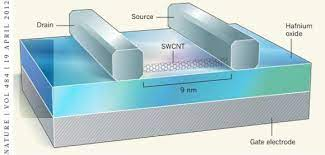
\includegraphics[scale=0.3]{IMAGENES/image1.jpg}
			\end{enumerate} &
			\begin{enumerate}
				\item[]\textbf{CMOS}
				\item FET basados en silicio tienen mayor retardo, así como el voltaje de
				suministro lo es.
				\item Los dispositivos de silicio, si se redujeran al tamaño del dispositivo
				basado en nanotubos de carbono, aún seguirían siendo más lentos. 
				\vspace{3mm}
				\item[] \hspace*{10mm}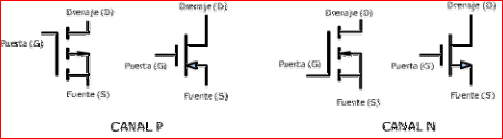
\includegraphics[scale=0.3]{IMAGENES/2.png}
			\end{enumerate}\\
			\hline
		\end{tabular}
		\caption{Nanotubos de carbono en comparación con los CMOS}
	\end{table}


%----------------- Diseño de fuentes de corrientes ---------------------
\section{Criterios de diseño de fuentes de corriente}
	La parte primordial de los amplificadores operacionales son los DA (differential amplifier), ya que este amplifica la diferencia de dos entredas de voltaje. Estos estan elaborados con tecnologias CMOS y los BIPOLARES, que con el tiempo se vio las deficiencias que presenta.
	\begin{itemize}
		\item Elevado consumo de energia
		\item Velocidad de tecnologia en los bipolares
		\item Los MOSFET en escalas de nano presenta limitaciones
	\end{itemize}
	En ese sentido se hace uso de los CNTFET (transistor de efecto de campo de nanotubos de carbono) que son los nuevas herramientas del futuro para los dispositivos electrónicos.\\
	Como menciona \cite{Akhoon}, CNTFET es un dispositivo prometedor y se puede utilizar para extender la validez de la ley más conocida de Gordan Moore. Se ha encontrado que el CNTFET intrínseco tiene Características $CV/I \sim 13$ veces más altas que las de un convencional $n-MOSFET$, el transistor de efecto de campo de nanotubos de carbono (CNFET) es una excelente alternativa a un transistor a granel tradicional para bajo consumo de energía y alto rendimiento, según \cite{Liu}




	\begin{itemize}
		\item Reducción de potencia consumida 
		\item Alta velocidad de procesamiento
		\item Eficiencia en los circuitos integrados 
		\item Gran capacidad de conducción eléctrica 
		\item Alta resistencia a la tracción
		\item Conductividad térmica
	\end{itemize}

		Son laminas de grafeno enrollados en tubos, que presentan caracteristicas: 
		\begin{itemize}
			\item Eléctricas
			\item Mecánicas
			\item Semiconductoras
			\item Prop. optoelectrónicas
		\end{itemize}




	\begin{figure}[!h] 
		\centering
		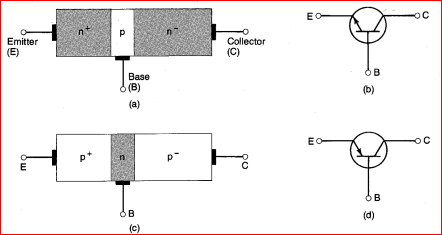
\includegraphics[scale=0.7]{IMAGENES/1.PNG}
		\caption{Estructura interna de los nanotubos de carbono \cite{Prasad}}
		\label{f_4}
	\end{figure}
	De acuerdo a la figura \ref{f_4}, podemos observar que presenta 2 formas:
	\begin{itemize}
		\item Single wall carbone nanotube (SWCNT)
		\item Multi wall carbone nanotube (MWCNT)
	\end{itemize}



Diametro de los nanotubos
		\begin{equation}
			D_{CNT} =  \frac{\sqrt{3}a_0}{\pi}\sqrt{n^2 + m^2 + mn}
		\end{equation}
		Donde:
		\begin{itemize}
			\item n,m son los valores de vectores de quiralidad del nanotubo
			\item $a_0$ distancia interatómica entre cada átomo de carbono
		\end{itemize}

Voltaje umbral
		\begin{equation}
			V_{th}\approx \frac{E_g}{2e} = \frac{\sqrt{3}}{3}\frac{a V_{\pi}}{eD_{CNT}}
		\end{equation}
		\begin{itemize}
			\item $a= 2.49A$, distancia de carbono a átomo de carbono
			\item $V_{\pi} = 3.033eV$ energía de enlace del carbono
			\item $e$, es el valor de la carga del electrón
		\end{itemize}

	




Ancho de banda
		\begin{equation}
			W = (N-1)S+D_{CNT}
		\end{equation}
		\begin{itemize}
			\item N, números de CNTS
			\item S, es la distancia entre el centro de dos CNTs (factor importante para el diseño)
		\end{itemize}
		\textbf{\textit{La influencia de varios parámetros de $CNTFET$, N, S y $D_{CNT}$}}

	\begin{figure}[!h] 
		\centering
		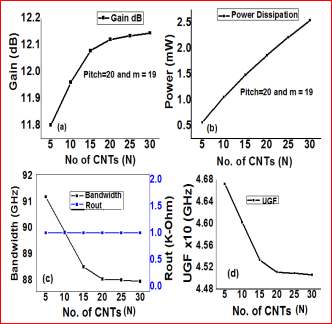
\includegraphics[scale=0.5]{IMAGENES/4.PNG}
		\caption{Variación de (a) Ganancia de corriente (b) Disipación de potencia (c) Ancho de banda (d) Frecuencia de ganancia unitaria con N en la propuesta basada en CNT-DA\cite{Akhoon}}
	\end{figure}




	\begin{figure}[!h] 
		\centering
		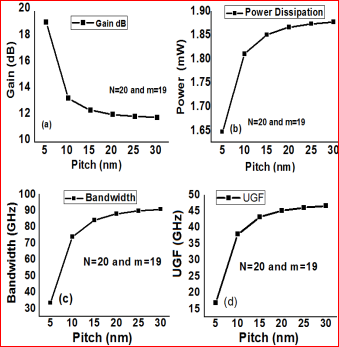
\includegraphics[scale=0.8]{IMAGENES/5.PNG}
		\caption{Variación de (a) ganancia de corriente (b) Disipación de potencia (c) Ancho de banda (d) Frecuencia de ganancia unitaria con respecto al tono de CNT-DA \cite{Akhoon}}
	\end{figure}




	\begin{figure}[!h] 
		\centering
		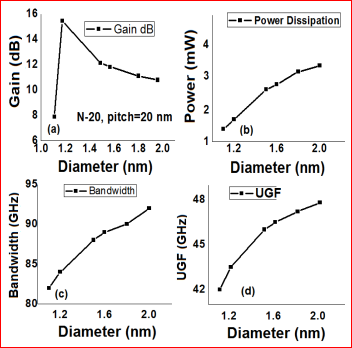
\includegraphics[scale=0.8]{IMAGENES/6.PNG}
		\caption{Variación de (a) Ganancia (b) Disipación de potencia (c) Ancho de banda (d) Frecuencia de ganancia unitaria con respecto al diámetro de CNT-DA \cite{Akhoon}}
	\end{figure}


%-------------------- Fuentes de corrientes --------------------------


\section{Fuentes de corrientes}
Algunas fuentes de corrientes
	\begin{itemize}
		\item Fuente de corriente constante cascode
		\item Fuente de corriente constante con FET(Mosfet)
	\end{itemize}


\subsection{Fuente de corriente constante cascode}


	Una forma de eliminar la disparidad de $V_{DS}$ es usar la configuración
	cascode:
	\begin{figure}[!ht]
		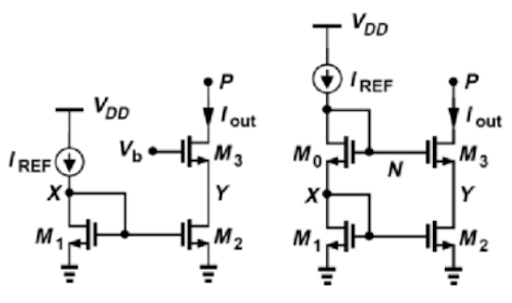
\includegraphics[scale=0.3]{IMAGENES/image3.png}
	\end{figure}
	$V_{DD}$ tal que $V_X = V_Y$
	$$\dfrac{\left(\dfrac{W}{L}\right)_3}
	{\left(\dfrac{W}{L}\right)_0} = 
	\dfrac{\left(\dfrac{W}{L}\right)_2}
	{\left(\dfrac{W}{L}\right)_1}$$ 
	
	donde
	\begin{center}
		\hspace{-5mm}W: ancho de puerta\\
		L: longitud de la puerta
	\end{center}



	\begin{align}
		V_{P_{min}} &= V_{DS_{sat_{2}}} + V_{DS_{sat_3}} \\
		V_{P_{min}} &= (V_{GS_0} - V_{TH_0}) + (V_{GS_1} - V_{TH_1}) \\
		V_{P_{min}} &= 2V_{DS_{sat}} + V_{TH_3} = 2V_{OD} + V_{TH} \\
	\end{align}
	Dimensionando correctamente los transistores logramos que $M_3$
	absorba las variaciones de $V_P$ y mantenga $V_X = VY$.\newline
	
	Por debajo de la tensión mínima de salida, $M_3$ ya no puede 
	absorber las diferencias de $V_{DS}$ y $V_B$ y será distinto a 
	$V_A$, volviendo a los problemas de espejo simple. Para tensiones
	muy bajas, la resistencia de salida se degrada.
	
	\begin{figure}
		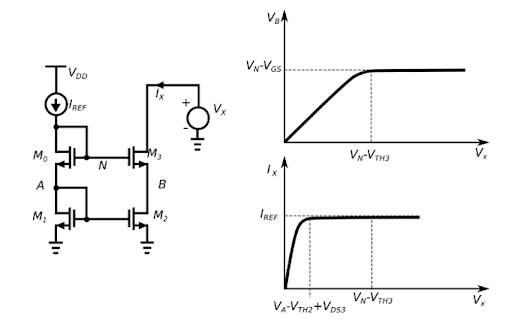
\includegraphics[scale=0.3]{IMAGENES/image4.png}
	\end{figure}


\subsection{Fuente con FET}


			\begin{itemize}
				\item El par diferencial básico consta de dos MOSFET de enriquecimiento acoplados ($Q_1$ y $Q_2$), polarizados con una fuente de corriente constante; esta ultima suele ser una configuración de espejo de corriente similar a la utilizada con BJT’s. desde luego se supone que el circuito de carga es tal que los dos MOSFET que conforman el par, se encuentran operando en la región de saturación.
				\item El MOSFET es frecuentemente usado como amplificador de potencia y ofrece como ventaja una resistencia de entrada alta, prácticamente infinita en la compuerta y una corriente de polarización de entrada cai cero.
				\item Existen dos razones fundamentales por las cuales se prefieren los amplificadores diferenciales sobre los de un solo extremo: son sensibles a la interferencia y no necesitan capacitores de paso y acoplamiento.
			\end{itemize}

			\begin{figure}[!ht]
				\centering
				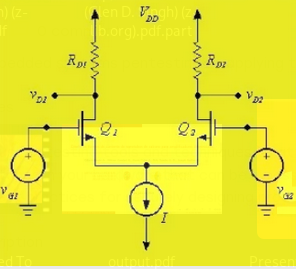
\includegraphics[width=5cm]{IMAGENES/image5.png}
				\caption{Amplificador diferencial con FETs}
			\end{figure}




	\section{Conclusiones}
	

				\begin{itemize}
					\item Las fuentes de corrientes   basados en nanotubos de carbono y FETs tienen ventajas por encima que los BJTs: no dependen de hie, por ende no se verán afectados por la temperatura.
					\item Las fuentes de corrientes se usan en los amplificadores de corriente como un elemto de amplificador, ya que fijará un valor constante para el punto de operación del amplificador diferencial.
				\end{itemize}





 

%%%%%%%%%%%%%%%%%%%%%%%%%%%%%%%%%%%%%%%%%%%%%%%
%%%%%
%%%%%   BIBLIOGRAFÍA     %%%%%%%%%%%%%%%%%%%%%%
%%%%%
%%%%%%%%%%%%%%%%%%%%%%%%%%%%%%%%%%%%%%%%%%%%%%%

\bibliographystyle{ieeetr}
\bibliography{bibliografia}

\end{document}
